
\chapter{Spectrum by Quantum Walk}

In this chapter, the Spectrum by Quantum Walk algorithm, proposed by \textcite{poulin}, is discussed. \todo{make bigger}

\section{Operators of the Algorithm}
The starting point of this algorithm is the Hamiltonian of the system aimed to simulate:

$$
H = \sum_{j=0}^N \alpha_j P_j.
$$
This Hamiltonian is sum of $N$ multi-qubit Pauli operator multiplied by some real coefficient. Unlike the sum of the second-quantized Hamiltonian in equation \ref{quant}, the number of terms here does not have a direct physical meaning, but is rather dependent on the Jordan-Wigner, Bravyi-Kitaev or parity encoding. A multi-qubit Pauli operator is a tensor product of the four Pauli operators $\set{I, X, Y, Z}. $

Before we move forward, we must ensure that the Hamiltonian we are working with is normalized, as we will map the coefficients to a quantum register in the algorithm. We do so by introducing a scaling factor of $\mathcal{N} = \sum_{j=0}^N |\alpha_j|$ \cite{poulin}. We absorb the sign of the coefficients into $P_j$.

Then our new, rescaled Hamiltonian, which we will call $\bar{H}$, takes the following form:

\begin{equation}
	\bar H = \frac H{\mathcal{N}} = \sum_j|\beta_j|^2 P_j,
\end{equation}

where $\beta_j = \sqrt{|\alpha_j|/\mathcal{N}}$. Due to the nature of the scaling factor $\mathcal{N}$,   $\sum_j \abs{\beta_j}^2 = 1.$ The eigenstates and eigenvalues of the rescaled Hamiltonian are

\begin{equation}
	 \bar{H} \ket{\phi_k} = \bar{E_k} \ket{\phi_k}.
\end{equation}

The Hamiltonian acts on the $n$ qubits required to store the wavefunction of the system and its matrix representation has dimension $2^n \times 2^n$. It therefore also has $2^n$ eigenvalue/eigenstate pairs. Since we do not know the exact value of the eigenvalue or eigenstate, we generalize by referring to some eigenstate with the subscript $k$, where $k = 0$ refers to the ground state.

Later we will define the operator $W$. This operator will act on two registers, the \verb|ancillary| register and the \verb|physical| register. We shall soon define certain unitary operations of the form $A\otimes B$, in which $A$ will act on the \verb|ancillary| register and $B$ on the physical register. Following \textcite{poulin}, we define $\ket{\beta}$ to be the state that results from applying $B$ to the zero-state.

$$
\ket{\beta} = B\ket{0} = \sum_j \beta_j \ket{j},
$$
where $\sum_j \beta_j$ are the coefficients from equation 3.1.
Later, we will initialize the \verb|ancillary| register in the state $\ket{\beta}$. Remember that $\beta_j$ are the coefficients of the rescaled Hamiltonian, so the bit string basis states $\ket{j}$ are in one-to-one correspondence with the coefficients of the Hamiltonian. As the sum of $\beta_j$ is normalized, the resulting state $\ket{\beta}$ is in superposition of the $N$ basis states, depending on the coefficients of the multi-qubit Pauli operators of the Hamiltonian. Next, we define the tranformations $S$ and $V$ as
\begin{equation}
S = (B (I - 2 \ket{0}\bra{0}) B^{\dagger}) \otimes I= (I-2\kb \beta \beta) \otimes I,
\end{equation}
\\
\begin{equation}
V=\sum_{j}\ket{j}\bra{j} \otimes P_{j}.
\end{equation}

These operations are unitary, which we will prove now.

\begin{align} \begin{split}
SS^{\dagger} &= ((I-2\kb \beta \beta) \otimes I)^{\dagger}((I-2\kb \beta \beta) \otimes I)\\
&= (I-2\kb \beta \beta)^{\dagger}(I-2\kb \beta \beta) \otimes I^2 \\
&= (I - 2 (\kb \beta \beta)^{\dagger})(I-2\kb \beta \beta)\\ \text{ As } (AB)^{\dagger} = B^{\dagger}A^{\dagger},\\
&= (I - 2 \bra{\beta}^{\dagger} \ket{\beta}^{\dagger})(I-2\kb \beta \beta) text{ as } (AB)^{\dagger} = B^{\dagger}A^{\dagger}.\\
&= (I-2\kb \beta \beta)(I-2\kb \beta \beta)\\
&= I - 4 \kb \beta \beta + 4 \ket{\beta}\braket{\beta}{\beta} \bra{\beta}\\
&= I - 4 \kb \beta \beta + 4 \ket{\beta} \sum_l B_l^{\dagger} \sum_j B_j \braket{l}{j}  \bra{\beta}\\
\end{split} \end{align}
\todo{mathintotext}

We will take this opportunity to introduce an identity for the inner product of $\beta$ and bit-string states. The following holds true for $\beta$:

$$ \braket{\beta}{\beta} = \sum_l B_l^{\dagger} \sum_j B_j \braket{l}{j} =  \sum_{l,j} B_l^{\dagger} \sum_j B_j \delta_{lj} = 1. $$

Such inner products will appear many times in the following sections. Continuing the proof of unitarity of $S$,

$$S S^{\dagger} = I - 4 \kb \beta \beta + 4 \ket{\beta} \bra{\beta} = I.$$

The unitarity of $V$ is proven similarly:

\begin{align} \begin{split}
VV^{\dagger} &= (\sum_{j} \kb jj \otimes P_{j})^{\dagger} \cdot \sum_{j} \kb jj \otimes P_{k} \\
&= \sum_{j} \kb jj \otimes P_{j} \cdot \sum_{j} \kb jj \otimes P_{j} \text{as}  P^{\dagger}_j = P_j.\\
&= \sum_j \kb jj  \otimes P_j^2\\
& \text{\  As  \ } \sum_{j}^{n} \kb jj = I \text{ and} \sum_j P_j^2 = I,\\
& VV^{\dagger} = I \\
\end{split} \end{align}


\section{Orthonormal bases}
\textcite{poulin} postulate the following orthonormal basis, in which $S$ and $V$ preserve the subspace spanned by that basis, which will be the same substate that $W$ will be initialized to:

\begin{align} \begin{split} \label{basis}
\ket{\varphi_k^0} &= \sum_j\beta_j\ket j\otimes\ket{\phi_k}, \\
\ket{\varphi_k^1} &= \frac 1{\sqrt{1-E_k^2}}(V-E_k)\ket{\varphi_k^0}.
\end{split} \end{align}
Here, $E_k$ is the energy corresponding to the $k$-th eigenstate of the Hamiltonian, $\ket{\phi_k}$. In this section, we prove that above basis states are normalized and orthogonal. In these proofs, inner products of the Hamiltonian eigenstates will appear. As these eigenstates are orthogonal, the inner product becomes:

\begin{equation}
	\braket{\phi_{k'}}{\phi_k} = \delta_{k'k}.
\end{equation}

In this thesis, we assume that $ k' = k$, unless specified otherwise. First, we show that $\ket{\varphi_k^0}$ is normalized by taking the inner product with itself:

\begin{align} \begin{split}
\braket{\varphi_k^0}{\varphi_k^0}  &= (\bra{\beta} \otimes \bra{\phi_k})(\ket{\beta} \otimes \ket{\phi_k})\\
&= \braket{\beta}{\beta} \otimes \braket{\phi_k}{\phi_k}\\
&= 1.
\end{split} \end{align}

Similarly, we can show that $\ket{\varphi_k^1}$ is normalized:
\begin{align} \begin{split}
\braket{\varphi_k^1}{\varphi_k^1}  &= \bra{\varphi_k^0} \frac{1}{\sqrt{1 - E^2_k}}(V-E_k) \frac{1}{\sqrt{1 - E^2_k}}(V-E_k) \ket{\varphi_k^0}\\
&= \bra{\varphi_k^0} \frac{1}{1 - E^2_k} (V-E_k)^2  \ket{\varphi_k^0}\\
&= \frac{1}{1 - E^2_k} \bra{\varphi_k^0} (V^2 - 2 E_kV + E_k^2) \ket{\varphi_k^0}\\
&= \frac{1}{1 - E^2_k} \bra{\varphi_k^0} (I - 2 E_kV + E_k^2) \ket{\varphi_k^0}\\
\end{split} \end{align}

One term in this expression is the expectation value of $V$ in the $\ket{\varphi_k^0}$-basis. As finding the expectation value is slightly involved, we first show the proof of the expectation value before continuing with the normalization proof:
\begin{align} \begin{split}
\bra{\varphi_k^0} V \ket{\varphi_k^0} &= \bra{\varphi_k^0} (\sum_j \kb j j \otimes P_j) \sum_l \beta_l \ket{l} \otimes \ket{\phi_k}\\
&= \bra{\varphi_k^0}\sum_j \sum_l \beta_l \ket{j} \braket{j}{l} \otimes P_j \ket{\phi_k}\\
&=(\sum_m \beta_m^* \bra{m} \otimes \bra{\phi_k}) \sum_j \sum_l \beta_l \ket{j} \delta_{j,l} \otimes P_j \ket{\phi_k}\\
&= \sum_m \sum_j \beta_m^* \beta_j \braket{m}{j} \otimes \braket{\phi_k}{P_j \phi_k}\\
&= \sum_m \sum_j \beta_m^* \beta_j \delta_{m,j} \otimes \braket{\phi_k}{P_j \phi_k}\\
&= \sum_j \abs{\beta_j}^2 \braket{\phi_k}{P_j \phi_k}\\
&= \sum_j \braket{\phi_k}{\abs{\beta_j}^2 P_j \phi_k}.
\end{split} \end{align}

As $\bar{H}\ket{\phi_k} = E_k\ket{\phi_k}$ and $\bar{H} = \sum_j \abs{\beta_j}^2  P_j,$ we have that:
\begin{equation} \label{0V0}
\bra{\varphi_k^0} V \ket{\varphi_k^0} = \braket{\phi_k}{E_k \phi_k}
= E_k.
\end{equation}

We can now continue the proof of orthonormality of $\ket{\varphi_k^1}$ where we left off, using equation \ref{0V0}. The expression becomes:



\begin{align} \begin{split}
\braket{\varphi_k^1}{\varphi_k^1} &= \frac{1}{1 - E^2_k} \bra{\varphi_k^0} (I - 2 E_kV + E_k^2) \ket{\varphi_k^0}\\
&= \frac{1}{1 - E^2_k} \bra{\varphi_k^0} (I - 2 E_k^2 + E_k^2) \ket{\varphi_k^0}\\
&= \frac{1}{1 - E^2_k} \bra{\varphi_k^0} (I -  E_k^2) \ket{\varphi_k^0}\\
&= \frac{1- E^2_k}{1 - E^2_k} \braket{\varphi_k^0}{\varphi_k^0}\\
&= 1.
\end{split} \end{align}

Finally, we prove that the two basis states are orthogonal,  using equation \ref{0V0}:
\begin{align} \begin{split}
\braket{\varphi_k^0}{\varphi_k^1} &= \bra{\varphi_k^0}  \frac{1}{\sqrt{1 - E^2_k}}(V-E_k) \ket{\varphi_k^0}\\
&= \bra{\varphi_k^0}  \frac{1}{\sqrt{1 - E^2_k}}(E_k-E_k) \ket{\varphi_k^0}\\
&= 0.
\end{split} \end{align}

\subsection{Blockdiagonality}

The unitary property of $S$ and $V$ allow them to be put in block diagonal form with $ 2 \times 2$ blocks \cite{poulin}. A general block diagonal matrix only has nonzero entries in the blocks of size $n \times n$ on the diagonal, which for $n = 2$ looks like the following:

\[
\left(\begin{array}{@{}c|c@{}}
  \begin{matrix}
  a & b \\
  c & d
  \end{matrix}
  & \begin{matrix}
  0 & 0 \\
  0 & 0
  \end{matrix} \\
\hline
  \begin{matrix}
    0 & 0 \\
    0 & 0
    \end{matrix} &
  \begin{matrix}
  e & f \\
  g & h
  \end{matrix}
\end{array}\right).
\]

We can put the expectation values of $S$ and $V$ in one of such matrices in the space of $\ket{\varphi_k^0}$ and $\ket{\varphi_k^1}$. Putting the operators $S$ and $V$ into block diagonal form with placeholder values in aforementioned space creates the following structure:
\begin{equation}
\kbordermatrix{&
\ket{\varphi_0^0}&\ket{\varphi_0^1}&\vrule&\ket{\varphi_1^0}&\ket{\varphi_1^1}&\vrule&\cdots&\vrule&\ket{\varphi_k^0}&\ket{\varphi_k^1}\\
\bra{\varphi_0^0}&V_{11}&V_{21}&\vrule&0&0&\vrule&&\vrule&0&0\\
\bra{\varphi_0^1}&V_{12}&V_{22}&\vrule&0&0&\vrule&&\vrule&0&0\\\hline
\bra{\varphi_1^0}&0&0&\vrule&V_{33}&V_{43}&\vrule&&\vrule&0&0\\
\bra{\varphi_1^1}&0&0&\vrule&V_{43}&V_{44}&\vrule&&\vrule&0&0\\\hline
\vdots&&&\vrule&&&\vrule&\ddots&\vrule\\\hline
\bra{\varphi_k^0}&0&0&\vrule&0&0&\vrule&&\vrule&V_{ii}&V_{ij}\\
\bra{\varphi_k^1}&0&0&\vrule&0&0&\vrule&&\vrule&V_{ji}&V_{jj}\\
}
\end{equation}

The off-diagonal elements are zero as $ \braket{\phi_k}{\phi_l} = \delta_{k,l}$. As the expectation values of $S$ and $V$ in the basis defined in \ref{basis} will be useful later in this thesis, we shall now try to find these values.  Before we do so, it will be convenient to first find the result of $S$ applied to $\ket{\varphi_k^0}$:

\begin{align} \begin{split}
  \label{sket}
  S \ket{\varphi_k^0} &= ((I - 2\dyad{\beta}{\beta}) \otimes I) \ket{\beta} \otimes \ket{\phi_k}\\
  &= \ket{\beta} \otimes \ket{\phi_k} - 2 \ket{\beta} \otimes \ket{\phi_k}\\
  &= - \ket{\varphi_k^0}.
\end{split} \end{align}

Then the expectation value of $S$ in $\ket{\varphi_0^0}$ simply becomes:

\begin{align} \begin{split}
\bra{\varphi_0^0}S\ket{\varphi_0^0} &= \bra{\varphi_0^0} \left( - \ket{\varphi_k^0} \right)\\
&= - \braket{\varphi_0^0}{\varphi_0^0}\\
&= - 1.
\end{split} \end{align}

Next, we find the expectation value of the offdiagonal entries in the matrix:

\begin{align} \begin{split}
\bra{\varphi_0^0}S\ket{\varphi_0^1} &= \bra{\varphi_0^0} \left(- \ket{\varphi_0^1}\right) \text{using \ref{sket}}\\
&= - \bra{\varphi_0^0} \ket{\varphi_0^1}\\
&= 0.
\end{split} \end{align}

Because the operator $S$ is symmetric around the diagonal, it is self adjoint and from the identity \cite{nielsen} $$\bra{\psi} A^{\dagger}\ket{\phi}= \bra{\phi} A \ket{\psi}^{*}$$
we can conclude that $\bra{\varphi_0^0}S\ket{\varphi_0^1} = \bra{\varphi_0^1}S\ket{\varphi_0^0} = 0.$

\begin{align} \begin{split}
\bra{\varphi_0^1}S\ket{\varphi_0^1} &= \fr \bra{\varphi_0^1} S(V-E_k) \ket{\varphi_0^0} \\
&= \fr \bra{\varphi_0^1} SV - S E_0 \ket{\varphi_0^0})\\
&= \fr ( \bra{\varphi_0^1} SV \ket{\varphi_0^0} + E_k \bra{\varphi_0^1} S \ket{\varphi_0^0})\\
&= \fr \bra{\varphi_0^1} SV \ket{\varphi_0^0} \\
&= \fr \bra{\varphi_0^1} (I - 2 \kb \beta \beta) V \ket{\varphi_0^0}\\
&= \fr ( \bra{\varphi_0^1} V \ket{\varphi_0^0} - 2  \bra{\varphi_0^1} \kb \beta \beta V \ket{\varphi_0^0})\\
&= \frac{\sqrt{1-E_0^2}}{\sqrt{1-E_0^2}} - 2 \fr \bra{\varphi_0^1} \sum_j \abs{\beta_j}^2 \ket{\beta} \otimes P_j \ket{\phi_0}\\
&= 1 - \frac{2}{\sqrt{1-E_0^2}} \bra{\varphi_0^1} \left(\ket{\beta} \otimes H \ket{\phi_0}\right)\\
&= 1 - \frac{2E_k}{\sqrt{1-E_0^2}} \bra{\varphi_0^1} \left(\ket{\beta} \otimes \ket{\phi_0}\right)\\
&= 1 - \frac{2E_k}{\sqrt{1-E_0^2}} \bra{\varphi_0^1} \ket{\varphi_0^0}\\
&= 1.
\end{split} \end{align}



The block-diagonal matrix of $S$ is now completed, and has the following form:

\begin{equation}
S = \
\kbordermatrix{& \ket{\varphi_0^0}&\ket{\varphi_0^1}\\
\bra{\varphi_0^0}&-1&0\\
\bra{\varphi_0^1}&0&1}.
\end{equation}

Since there is no $k$-dependency, this matrix can be generalised for all $k$-values, which gives the following:


\begin{equation}
S = \
\kbordermatrix{& \ket{\varphi_k^0}&\ket{\varphi_k^1}\\
\bra{\varphi_k^0}& -1&0\\
\bra{\varphi_k^1}&0&1\\
}.
\end{equation}


Let us find the equivalent matrix for the operator $V$. In equation \ref{0V0}, it has been shown that $\bra{\varphi_k^0} V \ket{\varphi_k^0} = E_k$. Next, we find the off-diagonal elements:

\begin{align} \begin{split}
\bra{\varphi_0^0}V\ket{\varphi_0^1}&= \bra{\varphi_0^0}  \frac{1}{\sqrt{1 - E^2_0}} (V^2 - E_0V) \ket{\varphi_0^0}\\
&= \frac{1}{\sqrt{1 - E^2_0}} \left( \braket{\varphi_0^0}{\varphi_0^0} - E_0 \bra{\varphi_0^0} V \ket{\varphi_0^0}\right)\\
&=  \left( \braket{\varphi_0^0}{\varphi_0^0} - E_0^2 \bra{\phi_0} \ket{\phi_0}\right) \text{ using \ref{0V0}}\\
&= \sqrt{1 - E^2_0}.
\end{split} \end{align}

As $V$ is also symmetric and therefore self-adjoint, $$\bra{\psi} A^{\dagger}\ket{\phi}= \bra{\phi} A \ket{\psi}^{*}$$ holds again and thus $$\bra{\varphi_0^0}V\ket{\varphi_0^1} = \bra{\varphi_0^1}V\ket{\varphi_0^0} = \sqrt{1 - E^2_0}.$$

Lastly, we need to find $\bra{\varphi_0^1}V\ket{\varphi_0^1}$:

\begin{align} \begin{split}
\bra{\varphi_0^1}V\ket{\varphi_0^1} &= \bra{\varphi_0^1}  V\frac{V- E_0}{\sqrt{1 - E^2_0}} \ket{\varphi_0^0}\\
&= \bra{\varphi_0^0} \frac{1}{1 - E^2_0} (V - E_0)(1 - E_0V)\ket{\varphi_0^0}\\
&= \bra{\varphi_0^0} \frac{1}{1 - E^2_0} (V - E_0 - E_0 + E_0^2V)\ket{\varphi_0^0} \text{ using equation \ref{0V0}}\\
&= \bra{\phi_0} \frac{1}{1 - E^2_0} (-E_0 + E_0^3)\ket{\phi_0}\\
&= \bra{\phi_0} \left(- E_0 \frac{1 - E^2_0}{1 - E^2_0}\ket{\phi_0}\right)\\
&= \bra{\phi_0} \left(- E_0 \ket{\phi_0}\right)\\
&= - E_0.
\end{split} \end{align}

Once again, we can compile these values in the block matrix and generalize to any $k$-value in the range of energy states to obtain:

\begin{equation}
V = \
\kbordermatrix{& \ket{\varphi_k^0}&\ket{\varphi_k^1}\\
\bra{\varphi_k^0}& E_k&\sqrt{1 - E^2_0}\\
\bra{\varphi_k^1}&\sqrt{1 - E^2_0}&-E_k
}
\end{equation}
\newpage

\section{Creating the Unitary Walk Operator}

So far, we have defined three unitary operations ($B$, $S$ and $V$) and have defined an orthogonal basis $\{\ket{\varphi_k^0}, \ket{\varphi^1_k}\}$. $B$ is the ancillary state preparation operator, creating a superposition of states while incorporating the Hamiltonian coefficients. $S$ is a reflection operator and $V$ is a controlled operator that applies Pauli operators.
\textcite{poulin} define a unitary operator $W$ which preserves the subspace spanned by the orthogonal basis just specified:


% To see what effect $V$ has on a state in this subspace, we can simply apply $V$ to some state in the subspace. For efficiency reasons, we pick $c_0 = 1 \wedge c_1 = 0$.
%
% \begin{align} \begin{split}
% V \ket{\psi} &= V \ket{\varphi_k^0}\\
% &= \Vop \fiok\\
% &= \sum_j \beta_j \ket{j} \otimes P_j \ket{\phi_k}
% \end{split} \end{align}
%
% From this result, we conclude that $V$ applies the specific Pauli operator, corresponding to the state of the system of qubits, to the $k_{th}$ eigenstate of the Hamiltonian. \textcite{poulin} define the unitary walk operator as:

\begin{equation}
W = SV.
\end{equation}

As we have defined both $S$ and $V$ in the $\{\ket{\varphi_k^0}, \ket{\varphi^1_k}\}$-basis, we can find the block-diagonal matrix for $W$ as well:

\begin{align} \begin{split}
W = SV &=
\begin{array}{l}
\left(\begin{array}{cc}
-1 & 0 \\
0 & 1
\end{array}\right) \left(\begin{array}{cc}
E_{k} & \sqrt{1-E_{k}^{2}} \\
\sqrt{1-E_{k}^{2}} & -E_{k}
\end{array}\right)
\end{array} \\
&= \left(\begin{array}{cc}
-E_{k} & -\sqrt{1-E_{k}^{2}} \\
\sqrt{1-E_{k}^{2}} & -E_{k}
\end{array}\right). \end{split}
\end{align}

The operator $W$ has eigenstates $\ket{\varphi^{\pm}_k} = \ket{\varphi^0_k} \pm i \ket{\varphi^1_k}$ \cite{poulin}. Let us find the eigenvalues by applying $W$ to its eigenstates:

\begin{align}
  W \ket{\varphi^+_k} &= \frac{1}{\sqrt{2}}\left(W \ket{\varphi^0_k} + W i \ket{\varphi^1_k}\right)\\
  &= \frac{1}{\sqrt{2}} \left( SV \ket{\varphi^0_k} + i SV \frac{V-E_k}{\sqrt{1-E_k^2}} \ket{\varphi^0_k}\right)\\
  &= \frac{1}{\sqrt{2}} \left( SV \ket{\varphi^0_k} + \frac{iS}{\sqrt{1-E_k^2}} I \ket{\varphi^0_k} - \frac{i E_k}{\sqrt{1-E_k^2}} SV \ket{\varphi^0_k}\right)\\
  &= \frac{1}{\sqrt{2}} \left( \tm{\sqrt{1-E_k^2}S - i E_k S}V\ket{\varphi^0_k} + \tm{iS} \ket{\varphi^0_k} \right).
  \intertext{We want to obtain a factor of $ \ket{\varphi_k^1}$. To do so, we add and subtract a factor of $$E_k \left(\tm{\sqrt{1-E_k^2}S - i E_k S}\ket{\varphi^0_k}\right)$$ to obtain the desired $(V-E_k)$ factor in the left term of the equation above. Then, the expression becomes:}
  W \ket{\varphi^+_k} &= \frac{1}{\sqrt{2}} \left( \tm{\sqrt{1-E_k^2}S - i E_k S}(V-E_k)\ket{\varphi^0_k} + \tm{iS} \ket{\varphi^0_k} + E_k \tm{\sqrt{1-E_k^2} - i E_k } S\ket{\varphi^0_k} \right)
  \intertext{Given $\tm{V-E_k} \ket{\varphi^0_k} = \ket{\varphi^1_k}$ we obtain the following}
  &= \frac{1}{\sqrt{2}} \left( \left(\sqrt{1-E_k^2} - i E_k \right) S \ket{\varphi^1_k} + \tm{i + E_k(\sqrt{1-E_k^2} - i E_k)}S \ket{\varphi^0_k} \right).
  \intertext{Since $S \ket{\varphi^1_k} = \ket{\varphi^1_k}$ and $S\ket{\varphi^0_k} = -\ket{\varphi^0_k}$, our expression becomes}
  &= \frac{1}{\sqrt{2}} \left( \left(\sqrt{1-E_k^2} - i E_k \right) \ket{\varphi^1_k} - \left(E_k \frac{\sqrt{1-E_k^2}}{\sqrt{1-E_k^2}} + i\tm{1-E_k^2}\right) \ket{\varphi^0_k} \right)\\
  &=  \frac{1}{\sqrt{2}} \left( \left(\sqrt{1-E_k^2} - i E_k \right) \ket{\varphi^1_k} - \left( E_k + i \sqrt{1-E_k^2} \right)  \ket{\varphi^0_k} \right)\\
  &=  \frac{1}{\sqrt{2}}\left(\sqrt{1-E_k^2} - i E_k \right) \ket{\varphi^1_k} + \frac{1}{\sqrt{2}} \left(- E_k - i \sqrt{1-E_k^2} \right) \ket{\varphi^0_k}.\\
  \intertext{Following \textcite{steiger}, we can factor the coefficients of the basis state into $-E_k - i\sqrt{1-E_k^2}$ and obtain}
  &= \left(-E_k - i \sqrt{1-E_k2} \right) \frac{1}{\sqrt{2}} (\ket{\varphi_k^0} + i \ket{\varphi_k^1})\\
  &= \left(-E_k - i\sqrt{1-E_k2} \right) \ket{\varphi_k^+}.
  \intertext{As $E_k = \cos(\theta_k)$ (which we show in section 3.4) and $\abs{\sin(\theta_k)} = \sqrt{1-\cos^2(\theta_k)}$, we can write this as}
  &= \left(- \cos \left(\theta_{k}\right)-i \sin \left(\theta_{k}\right)\right) \ket{\varphi^+_k}\\
  &= e^{i\left(\pi+\theta_{k}\right)} \ket{\varphi^+_k}. \end{align}

Similarly, we can find that $W \ket{\varphi^-_k} = e^{i\left(\pi-\theta_{k}\right)} \ket{\varphi^-_k}$, which implies that the eigenvalues of $W$ are $e^{i\left(\pi \pm \theta_{k}\right)}$.

\section{Quantum Phase Estimation}
\label{sec:pea}
In this section, we briefly outline the canonical quantum Phase Estimation Algorithm (PEA) as introduced by \textcite{nielsen}. The norm of eigenvalues of all unitary operators, such as the unitary operator $W$, is one and the eigenvalues can be written in the form $\exp{2\pi i \theta}$. This algorithm prepares the physical register in the $\{\ket{\varphi_k^0}, \ket{\varphi_k^1\}}$ subspace, as the set of eigenvalues of $W$ in this specific subspace is a function of the Hamiltonian \cite{poulin}. As the eigenvalues of $W$ are $e^{i\left(\pi \pm \theta_{k}\right)}$, we can conclude that the eigenstate of the Hamiltonian, which is $E_k$, is encoded in the phase of $W$. The exact relation between the two spectra is given by \textcite{Babbush_2018}, who describe the same method of spectral encoding of the Hamiltonian

\begin{equation}
\label{spectrum}
\operatorname{spectrum}(H)=\lambda \cos (\arg (\operatorname{spectrum}(\mathcal{W}))).
\end{equation}

Here, $\arg$ represents the argument function of complex analysis, and $\lambda$ is the rescaling factor, equal to $\mathcal{N}$ introduced in equation 3.1. We follow the convention introduced by \textcite{poulin}, where $E_k$ refers to the rescaled energy. Consequently, we can rewrite equation \ref{spectrum} as

\begin{equation}
\cos(\theta_k) = E_k.
\end{equation}
We can thus perform an energy measurement by performing phase estimation on $W$.\\

Phase estimation makes use of two registers: an ancillary register of size $t$ and a system register, prepared in the eigenstate $\ket{u}$. We assume that the phase of the eigenvalue $\exp{2\pi i \varphi}$ can be written as a $0.\varphi_1 \varphi_2 ... \varphi_t$ in binary notation, where $t$ is the size of the ancillary register \cite{nielsen}. First, the qubits of the ancillary register is brought to an equal superposition through a Hadamard transform. Then, a series of controlled-$U$ operations are performed on the system register, where $U$ is raised to successive powers of two. The schematic circuit of this procedure can be seen in figure 3.1.

\begin{figure}[h] \label{peafig}
	\center 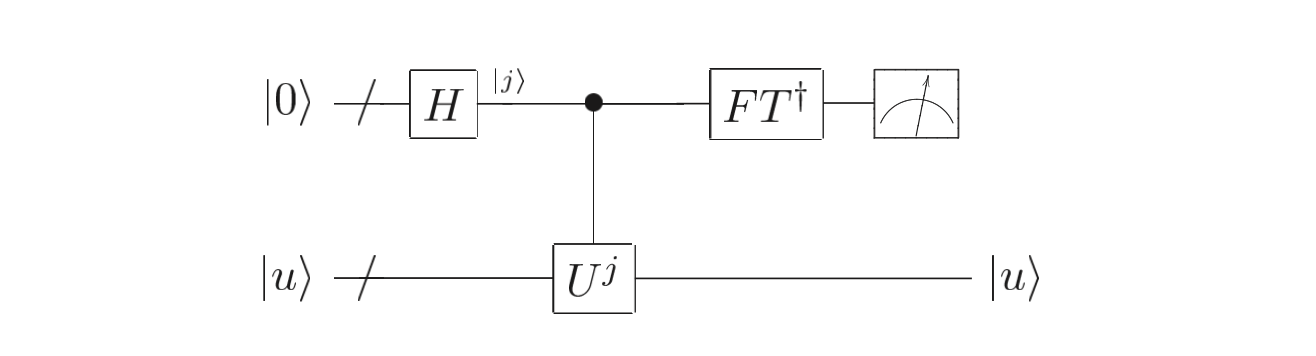
\includegraphics[width = \textwidth]{PEA.png}
	\caption{Schematic of the phase estimation procedure \cite[p.~223]{nielsen}.}
\end{figure}
\\
The state of the ancillary register after this procedure is

\begin{equation} \label{pea}
\frac{1}{2^{t / 2}} \sum_{k=0}^{2^{t}-1} e^{2 \pi i \varphi k}|k\rangle,
\end{equation}

where $\varphi$ is the phase of the eigenvalue of $U$. This first part of the phase estimation algorithm iteratively projects the phase of the unitary operator $U$ onto the state of the ancillary register. In order to retrieve the phase from the ancillary state, we must use the Fourier transform. The quantum Fourier transform is defined as \cite{nielsen}

\begin{equation}
|j\rangle \longrightarrow \frac{1}{\sqrt{N}} \sum_{k=0}^{N-1} e^{2 \pi i j k / N}|k\rangle,
\end{equation}

where $\ket{j}$ is a bit-string state and the sum is over an orthonormal basis $\ket{0},...,\ket{N-1}.$ From above definition and \hyperref{pea}, tt is clear that the ancillary state is the Fourier transform of the phase $\ket{\varphi_k}$. The next step of the phase estimation algorithm is to apply the inverse Fourier Transform ($FT^{\dagger}$ to the ancillary state:

\begin{equation}
\frac{1}{2^{t / 2}} \sum_{j=0}^{2^{t}-1} e^{2 \pi i \varphi j}|j\rangle|u\rangle \rightarrow|\tilde{\varphi}\rangle|u\rangle
\end{equation}

By applying a measurement in the computational basis, we now retrieve a good approximation of the phase, $\tilde{\varphi}$. Performing phase estimation on $W$ when the qubits are initialized to \(B|0\rangle \otimes\left|\tilde{\phi}_{0}\right\rangle\) gives $\pi \pm \theta_0$ with probability \(\left|\left\langle\phi_{0} | \tilde{\phi}_{0}\right\rangle\right|^{2}\). Then we can easily calculate the ground energy, as \(E_{0}=\cos \left(\pm \theta_{0}\right)\)
After the phase estimation process, the qubits are left in the eigenstate of $W$, $\ket{\varphi^{\pm}_k}$. Even though the furnished state is not directly the eigenstate of the Hamiltonian, we can still obtain relevant information of the eigenstate of the Hamiltonian. Since quantum states collapse upon measurement, we cannot simply measure a state once and define the superposition of that state. The general method to obtain information about a circuit or state is by performing repeated measurements of an hermitian observable $O$. Taking the average over these measurements, we obtain the expectation value of that observable:

$$
\bar{O}=\langle\varphi|O| \varphi\rangle.
$$ Similarly, we can find the expectation value of some observable in the eigenstate of $W$ and in the next section we prove that this gives us a value for the expectation values of observables in the Hamiltonian eigenstates themselves.
%As $U$ is unitary, it's eigenvalues are unitary as well and can therefore be written in the form $e^{i\theta_k}$. The eigenstates are $\ket{\varphi_k^\pm} = (\ket{\varphi_k^0} \pm i \ket{\varphi_k^1})/\sqrt 2$.



\section{Hamiltonian eigenstate expectation values}
Let $\sigma$ be some multi-qubit Pauli operator. The expectation value of $\sigma$ in the eigenstate of $W$ then can be written as the following.
\begin{align} \begin{split}
\bra{\varphi_k^{\pm}} \sigma \ket{\varphi_k^{\pm}} &= \left(\frac{1}{\sqrt{2}}\bra{\varphi_k^0} \mp i \bra{\varphi_k^1}\right) \sigma \left(\frac{1}{\sqrt{2}} \ket{\varphi_k^0} \pm i \ket{\varphi_k^1} \right)\\
&= \frac{1}{2}\left(\bra{\varphi_k^0} \sigma \ket{\varphi_k^0} \pm i \bra{\varphi_k^0} \sigma \ket{\varphi_k^1} \mp i \bra{\varphi_k^1} \sigma \ket{\varphi_k^0} + \bra{\varphi_k^1} \sigma \ket{\varphi_k^1}\right)\\
\end{split}\end{align}

We now consider each term individually.

\begin{align} \begin{split}
  \bra{\varphi_k^0} \sigma \ket{\varphi_k^0} &= \bra{\beta} \otimes \bra{\phi_k} \sigma \ket{\beta} \otimes \ket{\phi_k}\\
  &= \braket{\beta}{\beta} \otimes \bra{\phi_k} \sigma \ket{\phi_k}\\
  &= \bra{\phi_k} \sigma \ket{\phi_k}
\end{split} \end{align}



\begin{align} \begin{split}
  \bra{\varphi_k^0} \sigma \ket{\varphi_k^1} &=
  \frac{1}{\sqrt{1-E_k^2}} \bra{\beta} \otimes \bra{\varphi_k} \sigma (V - E_k) \ket{\beta} \otimes \ket{\phi_k}\\
  &=\frac{1}{\sqrt{1-E_k^2}} \bra{\beta} \otimes \bra{\varphi_k} \sigma ( \sum_j\beta_j \ket{j} \otimes P_j \ket{\phi_k} - E_k \ket{\beta} \otimes \ket{\phi_k})\\
  &= \frac{1}{\sqrt{1-E_k^2}}\left(\sum_j \abs{\beta_j^2} \bra{\phi_k} \sigma P_j\ket{\phi_k} - E_k \bra{\phi_k} \sigma \ket{\phi_k}\right)\\
  &= \frac{1}{\sqrt{1-E_k^2}}( E_k \bra{\phi_k} \sigma \ket{\phi_k} - E_k \bra{\phi_k} \sigma \ket{\phi_k})\\
  &= 0
\end{split} \end{align}

\begin{align} \begin{split}
  \bra{\varphi_k^1} \sigma \ket{\varphi_k^0} &= (\bra{\varphi_k^0} \sigma \ket{\varphi_k^1})^*\\
  &= 0
\end{split} \end{align}

\begin{align} \begin{split}
  \bra{\varphi_k^1} \sigma \ket{\varphi_k^1}) &=
  \frac{1}{1-E_k^2} \bra{\varphi_k^0} (V-E_k) \sigma (V-E_k) \ket{\varphi_k^0}\\
  &= \frac{1}{1-E_k^2} \bra{\varphi_k^0} (V \sigma V - V\sigma E_k - E_k \sigma V + E_k \sigma E_k )\ket{\varphi_k^0}\\
  &= \frac{1}{1-E_k^2} \bra{\varphi_k^0} V \sigma V \ket{\varphi_k^0} - \bra{\varphi_k^0} V\sigma E_k \ket{\varphi_k^0}\\
    &- \bra{\varphi_k^0} E_k \sigma V \ket{\varphi_k^0} + \bra{\varphi_k^0} E_k \sigma E_k \ket{\varphi_k^0})
\end{split} \end{align}

We once again consider each expectation value individually.

$$ \bra{\varphi_k^0} E_k \sigma E_k \ket{\varphi_k^0} = E_k^2 \bra{\phi_k} \sigma \ket{\phi_k} $$

Using equation 2.7, the following holds.
\begin{align} \begin{split}
\bra{\varphi_k^0} E_k \sigma V \ket{\varphi_k^0} &=  E_k\bra{\varphi_k^0} \sigma \ket{\beta} \otimes P_j \ket{\phi_k}\\
&= E_k \braket{\beta}{\beta} \otimes \bra{\phi_k} \sigma P_j \ket{\phi_k}\\
&= E_k \sum_j \bra{\phi_k} \sigma \abs{\beta_j}^2 P_j \ket{\phi_k}\\
&= E_k^2 \bra{\phi_k} \sigma \ket{\phi_k}
\end{split} \end{align}

As $\bra{\varphi_k^0} V \sigma E_k\ket{\varphi_k^0} $ is symmetric to $\bra{\varphi_k^0} E_k \sigma V \ket{\varphi_k^0}$, we can conclude that $\bra{\varphi_k^0} V \sigma E_k\ket{\varphi_k^0} = E_k^2 \bra{\phi_k} \sigma \ket{\phi_k}$


\begin{align} \begin{split}
  \bra{\varphi_k^0} V \sigma V \ket{\varphi_k^0} &= \bra{\beta}\otimes \bra{\phi_k} V \sigma V \ket{\beta} \otimes \ket{\phi_k}\\
  &= \sum_l \bra{l} \beta_l^{\dagger} \otimes \bra{\phi_k} P_l \sigma \sum_j \beta_j \ket{j} \otimes P_j \ket{\phi_k}\\
  &= \sum_j \abs{\beta_j}^2 \braket{j}{j} \otimes \bra{\phi_k} P_j \sigma P_j \ket{\phi_k}\\
  &= \sum_j \abs{\beta_j}^2  \bra{\phi_k} P_j \sigma P_j \ket{\phi_k}\\
\end{split} \end{align}

We split this sum up into two separate sums, where an extra constraint is placed on the (anti)commutation relation of $\sigma$ and $P_j$.

$$
&= \sum_{\substack{j \\ [\sigma, P_j = 0]}}\abs{\beta_j}^2  \bra{\phi_k} P_j \sigma P_j \ket{\phi_k} + \sum_{\substack{j \\ \{\sigma, P_j = 0\}}} \abs{\beta_j}^2  \bra{\phi_k} P_j \sigma P_j \ket{\phi_k}
$$

In the sum where $\sigma$ and $P_j$ commute, we can switch the order of $\sigma$ and $P_j$. We can do the same for the sum where $\sigma$ and $P_j$ commute, but that results in a sign change, as $AB = - BA$ for $ \{A,B\} = 0$. This gives

$$
&= \sum_{\substack{j \\ [\sigma, P_j = 0]}}\abs{\beta_j}^2  \bra{\phi_k} P_j  P_j \sigma \ket{\phi_k} - \sum_{\substack{j \\ \{\sigma, P_j = 0\}}} \abs{\beta_j}^2  \bra{\phi_k} P_j P_j \sigma \ket{\phi_k}.
$$

As $P_j$ is unconditionally unitary, $P^2_j = 1$. We can now merge the two sums back together by defining an additional operator \sigma:

$$\sigma \star P_j = 0 \iff [\sigma, P_j] = 0, \quad \sigma \star P_j = 1 \iff \{\sigma, P_j\} = 0.$$

Then the two sums can be written as
$$
\sum_{j}\left|\beta_{j}\right|^{2}(-1)^{\sigma \star P_{j}} \bra{\phi_k} \sigma \ket{\phi_k}
$$



%   &= \sum_j \abs{\beta_j}^2 \bra{\phi_k} P_j (P_j \sigma + [\sigma, P_j]) \ket{\phi_k}\\
%   \text{If $\sum_jP_j$ and $\sigma$ commute, then $[\sigma, ] = 0$ and}\\
%   &=  \sum_j \abs{\beta_j}^2 \bra{\phi_k} P_j^2 \sigma \ket{\phi_k}\\
%   &=  \sum_j \abs{\beta_j}^2 \bra{\phi_k} \sigma \ket{\phi_k}\\
%   & \text{If $P_j$ and $\sigma$ anticommute, then $[P_j, \sigma] =  2 P_j \sigma$ and}\\
%   &= \sum_j \abs{\beta_j}^2 \bra{\phi_k} P_j (P_j \sigma - 2 P_j \sigma) \ket{\phi_k}\\
%   &= \sum_j \abs{\beta_j}^2 \bra{\phi_k} - P_j^2 \sigma \ket{\phi_k}\\
%   &=  - \sum_j \abs{\beta_j}^2 \bra{\phi_k} \sigma \ket{\phi_k}.\\
% \end{split} \end{align}

Following the convention introduced by \textcite{poulin}, we define another variable $\Gamma$:
\begin{equation} \Gamma_{\sigma}=\sum_{j}\left|\beta_{j}\right|^{2}(-1)^{\sigma \star P_{j}}\end{equation}

Then the expectation value can be written as

\begin{equation}
  \bra{\varphi_k^0} V \sigma V \ket{\varphi_k^0} = \Gamma_{\sigma} \bra{\phi_k} \sigma \ket{\phi_k}
\end{equation}

Filling in the individual expecation values in equation 2.17, we obtain
\begin{align} \begin{split}
  \bra{\varphi_k^1} \sigma \ket{\varphi_k^1}) &= \frac{1}{1-E_k^2} (\bra{\varphi_k^0} V \sigma V \ket{\varphi_k^0} - \bra{\varphi_k^0} V\sigma E_k \ket{\varphi_k^0}\\
  &- \bra{\varphi_k^0} E_k \sigma V \ket{\varphi_k^0} + \bra{\varphi_k^0} E_k \sigma E_k \ket{\varphi_k^0})\\
  &= \frac{\Gamma_{\sigma} - 2 E_k^2 + E_k^2}{1-E_k^2} \bra{\phi_k} \sigma \ket{\phi_k}\\
  &=  \frac{\Gamma_{\sigma} - E_k^2}{1-E_k^2} \bra{\phi_k} \sigma \ket{\phi_k}.
\end{split} \end{align}

We can now fill this expression back in equation 2.13 and obtain the value for the expectation value of some multi-qubit Pauli operator in the $\varphi^{\pm}_k$-basis.


$$
\bra{\varphi_k^{\pm}} \sigma \ket{\varphi_k^{\pm}} = \frac{1}{2}(1+\frac{\Gamma_{\sigma} - E_k^2}{1-E_k^2})  \bra{\phi_k} \sigma \ket{\phi_k}
$$

Since $\Gamma_{\sigma}$ can be calculated classically, we obtain static expectation values without having to prepare the eigenstate of the Hamiltonian. However, while obtaining these expectation values is very useful, preparing the \verb|physical| register in the eigenstate of the Hamiltonian may also be desired. To do so, we apply $B^{\dagger}$ to the \verb|ancillary| register of the post-measurement state $\ket{\varphi_k^{\pm}}$, in which $\ket{\varphi_k}$ corresponds to the $E_k$ measured. This gives

\begin{align} \begin{split} \label{sup}
\left( B^{\dagger} \otimes I \right) \ket{\varphi_k^{\pm}} &= B^{\dagger} \left(\frac{1}{\sqrt{2}}\ket{\varphi_k^0} \mp i \ket{\varphi_k^1}\right) \\
&= \frac{1}{\sqrt{2}}(B^{\dagger} B \ket{0} \otimes \ket{\phi_k} \pm \left( B^{\dagger} \otimes I \right) i \ket{\varphi_k^1}\\
&= \frac{1}{\sqrt{2}}(\ket{0} \otimes \ket{\phi_k} \pm \left( B^{\dagger} \otimes I \right) i \ket{\varphi_k^1}\\
\end{split} \end{align}

The system can now be in two possible states: either the ancillary register is $\ket{0}$ and the physical register is in the desired state of $\ket{\phi_k}$, or the system is in $\left( B^{\dagger} \otimes I \right) i \ket{\varphi_k^1}$. According to \textcite{steiger}, the latter state has no overlap with the ancillary state $\ket{0}$, so the probability that the physical register is in the state $\ket{\phi_k}$ is $\frac{1}{2}$, given the superposition of \ref{sup}. We can then use an additional ancillary qubit to determine whether the ancilla register is in $\ket{0}$ without collapsing the system. We can achieve this by performing the operation described in \ref{xcx}, where the target qubit is the additional ancillary qubit, on which we perform a measurement afterwards. If this measurement returns 1, then the Hamiltonian eigenstate has been sucessfully prepared. Otherwise, we can apply
$B$ again and perform phase estimation of $W$ to return to $\ket{\varphi_k^{\pm}}$, where we can retry the process just described. Either way, we can prepare the ground state of the Hamiltonian without collapsing the state of the system.
